\documentclass[journal]{IEEEtran}

\usepackage{cite, graphicx}
\usepackage[usenames,dvipsnames]{xcolor}

% *** GRAPHICS RELATED PACKAGES ***
%
\ifCLASSINFOpdf
  % \usepackage[pdftex]{graphicx}
  % declare the path(s) where your graphic files are
  % \graphicspath{{../pdf/}{../jpeg/}}
  % and their extensions so you won't have to specify these with
  % every instance of \includegraphics
  % \DeclareGraphicsExtensions{.pdf,.jpeg,.png}
\else
  % or other class option (dvipsone, dvipdf, if not using dvips). graphicx
  % will default to the driver specified in the system graphics.cfg if no
  % driver is specified.
  % \usepackage[dvips]{graphicx}
  % declare the path(s) where your graphic files are
  % \graphicspath{{../eps/}}
  % and their extensions so you won't have to specify these with
  % every instance of \includegraphics
  % \DeclareGraphicsExtensions{.eps}
\fi

\usepackage[cmex10]{amsmath}
%\usepackage{algorithmic}
\usepackage{algorithm}
\usepackage{algorithmicx}
\usepackage{algpseudocode}
\usepackage{listings}

\usepackage{array,multirow,graphicx}
\usepackage{xspace}
\usepackage{amssymb, stmaryrd, algorithm, mathrsfs}
\usepackage{mdwmath}
\usepackage{mdwtab}
\usepackage{eqparbox}
\usepackage{lipsum}
%\usepackage[tight,footnotesize]{subfigure}
%\usepackage[caption=false]{caption}
%\usepackage[font=footnotesize]{subfig}
%\usepackage[caption=false,font=footnotesize]{subfig}

%\usepackage{fixltx2e}

\usepackage{stfloats}
%\usepackage{url}\newcommand{\urlb}[1]{{\color{blue}\url{#1}}}
\usepackage{color}
\usepackage{hyperref}
\hypersetup{
  colorlinks   = true, %Colours links instead of ugly boxes
  urlcolor     = blue, %Colour for external hyperlinks
  linkcolor    = blue, %Colour of internal links
  citecolor   = red %Colour of citations
}

\usepackage{amssymb}\newcommand{\todonote}[1]{\footnote{\color{red}TODO: #1}\marginpar[\color{red}\hfill$\blacktriangleright$]{\color{red}$\blacktriangleleft$\hfill}}

\newcommand{\csp}{\textsc{CSP}\xspace}
\newcommand{\cop}{\textsc{COP}\xspace}
\newcommand{\ghost}{\textsc{GHOST}\xspace}
\newcommand{\ie}{\textit{i.e.}}

\newcommand{\modelcsp}[4]%
{ \begin{trivlist}
  \item[]%
    \textbf{CSP model for #1}:\\
    \textit{Variables:} #2\\
    \textit{Domain:} #3\\
    \textit{Constraints:} #4
  \end{trivlist}%
}

\newcommand{\modelcop}[5]%
{ \begin{trivlist}
  \item[]%
    \textbf{COP model for #1}:\\
    \textit{Variables:} #2\\
    \textit{Domain:} #3\\
    \textit{Constraints:} #4
    \textit{Objectives:} #5
  \end{trivlist}%
}

% *** Do not adjust lengths that control margins, column widths, etc. ***
% *** Do not use packages that alter fonts (such as pslatex).         ***
% There should be no need to do such things with IEEEtran.cls V1.6 and later.
% (Unless specifically asked to do so by the journal or conference you plan
% to submit to, of course. )

% correct bad hyphenation here
\hyphenation{op-tical net-works semi-conduc-tor}

\begin{document}

% \lstset{
%   language=[ISO]C++,
%   basicstyle=\footnotesize,
%   keywordstyle=\color{red}\bfseries,
%   commentstyle=\color{violet}\textit,
%   stringstyle=\color{blue}\ttfamily
% }%,labelstyle=\tiny}


%
% paper title
% can use linebreaks \\ within to get better formatting as desired
\title{\ghost: A Combinatorial Optimization Solver for RTS-related Problems}
%
%
% author names and IEEE memberships
% note positions of commas and nonbreaking spaces ( ~ ) LaTeX will not break
% a structure at a ~ so this keeps an author's name from being broken across
% two lines.
% use \thanks{} to gain access to the first footnote area
% a separate \thanks must be used for each paragraph as LaTeX2e's \thanks
% was not built to handle multiple paragraphs
%

% \author{FirstName~LastName,~\IEEEmembership{Member,~IEEE,}
%         Jim~Raynor,~\IEEEmembership{Fellow,~RR,}
%         and~Sarah~Kerrigan,~\IEEEmembership{Life~Fellow,~ZS}% <-this % stops a space
% \thanks{FirstName~LastName is with the Department of Names
% GA, 30332 USA e-mail: (see http://www.michaelshell.org/contact.html).}% <-this % stops a space
% \thanks{J. Raynor and S. Kerrigane are with the Romeo\&Juliet Inc.}% <-this % stops a space
% \thanks{Manuscript received April 19, 2499; revised January 11, 2500.}}

\author{Florian~Richoux\thanks{Florian~Richoux is with the LINA of the Universit{\'e} de Nantes, France, and the JFLI of the University of Tokyo, Japan.},
        Jean-Fran{\c c}ois~Baffier\thanks{Jean-Fran{\c c}ois~Baffier is with the Department of Computing Science of the University of Tokyo, Japan.},
        Alberto~Uriarte\thanks{Alberto Uriarte is with the Computer Science Department at Drexel University, Philadelphia, PA, USA.}}



% note the % following the last \IEEEmembership and also \thanks - 
% these prevent an unwanted space from occurring between the last author name
% and the end of the author line. i.e., if you had this:
% 
% \author{....lastname \thanks{...} \thanks{...} }
%                     ^------------^------------^----Do not want these spaces!
%
% a space would be appended to the last name and could cause every name on that
% line to be shifted left slightly. This is one of those "LaTeX things". For
% instance, "\textbf{A} \textbf{B}" will typeset as "A B" not "AB". To get
% "AB" then you have to do: "\textbf{A}\textbf{B}"
% \thanks is no different in this regard, so shield the last } of each \thanks
% that ends a line with a % and do not let a space in before the next \thanks.
% Spaces after \IEEEmembership other than the last one are OK (and needed) as
% you are supposed to have spaces between the names. For what it is worth,
% this is a minor point as most people would not even notice if the said evil
% space somehow managed to creep in.

% The paper headers
\markboth{TCIAIG ~Vol.~X, No.~Y, Month~Year}%
{??? \MakeLowercase{\textit{et al.}}: \ghost: A Combinatorial Optimization Solver for RTS-related Problems}

\maketitle

\begin{abstract}
  This paper presents \ghost, a combinatorial optimization solver that
  an  RTS AI  developer can  use as  a blackbox  to solve  any problem
  encoded into a constraint satisfaction/optimization problem. We show
  how to model  three very different RTS problems,  each one belonging
  to   a   specific   level    of   abstraction,   by   a   constraint
  satisfaction/optimization problem and test our solver on them, using
  StarCraft as  a testbed. For  the three problems, \ghost  shows very
  good results computed within some tens of milliseconds.
\end{abstract}

\begin{IEEEkeywords}
Game   AI,   Real-Time   Strategy,  StarCraft,   CSP,   COP,   Solver,
Optimization, Combinatorics.
\end{IEEEkeywords}

% For peer review papers, you can put extra information on the cover
% page as needed:
% \ifCLASSOPTIONpeerreview
% \begin{center} \bfseries EDICS Category: 3-BBND \end{center}
% \fi
%
% For peerreview papers, this IEEEtran command inserts a page break and
% creates the second title. It will be ignored for other modes.
\IEEEpeerreviewmaketitle

\section{Introduction}\label{sec:intro}

\IEEEPARstart {O}{ne} can see games  as a simplification of the world:
The playground  is smaller, rules  are easier and less  numerous, thus
possibilities are  limited. However,  games are  still rich  enough to
propose complex, dynamic environments where  it remains difficult to a
computer  to make  predictions,  have a  global  understanding of  the
current situation  and then take  a decision. This is  especially true
when  information is  incomplete, forcing  the computer  to infer  the
global state of the game from  pieces of information. This is the case
with Real-Time Strategy  games, where a Clausewitz's fog  of war hides
the  opponent moves.   Thus, RTS  games  are very  suitable to  design
Artificial Intelligence techniques that  could be applied afterward in
other domains.

Many AI  techniques have  been used  in RTS  games. Without  making an
exhaustive  list,  we  can   cite  reinforcement  learning,  case-base
reasoning,  Bayesian  programming,   goal-driven  autonomy,  potential
fields, etc. We  recommend to the reader  surveys from Onta{\~n}{\'o}n
et       al.~\cite{OntanonSURCM13}       and       Robertson       and
Watson~\cite{RobertsonW14}  to have  a  very complete  overview of  AI
techniques in RTS games.

However, there are few works in RTS game AI using constraint programming
techniques,      in      particular     through      a      constraint
satisfaction/optimization problem  (\csp/\cop).  Among  others, branch
and  bound  algorithms have  been  used  to  optimize build  order  in
Churchill and Buro~\cite{ChurchillB11}.   Genetic algorithms have been
used off-line to  optimize build order, but  with multiple objectives,
analyzed  in Kuchem  et al.~\cite{KuchemPR13}  and a  population-based
algorithm has  been used for multi-objective  procedural aesthetic map
generation in  Lara-Cabrera et al.~\cite{LaraCF14}.   Still, \csp/\cop
offer a convenient, homogeneous framework  able to model a huge number
of combinatorial and optimization problems,  and propose a various set
of algorithms to solve these problems.

\csp/\cop are widely used in Artificial Intelligence to solve problems
like  path-finding, scheduling,  and  logistics.  Unlike  mathematical
programming, \csp/\cop  algorithms are  usually not designed  to solve
one  specific problem  but are  general, able  to manage  any problems
modeled with a \csp/\cop. Besides the  generality, it is also easy and
intuitive to model a problem  with a \csp/\cop. These altogether bring
ideal   conditions   to   design    and   develop   a   user-friendly,
easy-to-extend, general solver.



\subsection{RTS problem families}

Refer  to Onta{\~n}{\'o}n  et al.~\cite{OntanonSURCM13}  and Robertson
and Watson~\cite{RobertsonW14}.


\subsection{Goals and summary}

The research  presented in this  paper is  an extension of  Richoux et
al.~\cite{RichouxUO14},  where  the  problem  to  make  a  wall  at  a
chokepoint  in StarCraft  has been  modeled  and solved  thanks to  an
ad-hoc meta-heuristic algorithm.

The goal of this paper is double:
\begin{itemize}
\item  To present  to  the RTS  AI community  our  solver \ghost,  its
  architecture,  how  to model  different  problems  with it  and  the
  results we obtained.
\item To show that constraint  programming can be successfully used in
  RTS AI, at any level of abstraction.
\end{itemize}

It is organized as follows:  First in Section~\ref{sec:ghost}, we give
a     short    introduction     or    reminder     about    constraint
satisfaction/optimization problems,  how they model problems  and what
kind  of algorithms  exist to  solve  them.  Then,  we present  \ghost
architecture, what public is aimed, how  to use it to solve an already
encoded   problem   and  how   to   write   your  own   problems   via
\ghost.   Sections~\ref{sec:target},~\ref{sec:wall}   and~\ref{sec:bo}
give details about three different problem, each from a specific level
of abstraction (from the lower to the higher: Reactive Control, Tactic
and Strategy), how  we modeled them into a \csp/\cop  and what results
we  obtained by  applying  \ghost. Finally,  this  paper concludes  on
possible future works.

\section{\ghost:   A  General   meta-Heuristic  Optimization   Solving
  Tool}\label{sec:ghost}
\subsection{A brief introduction to \csp / \cop}

Constraint  Satisfaction Problems  (\csp) and  Constraint Optimization
Problems  (\cop)   are  two  close  formalisms   intensively  used  in
Artificial  Intelligence  to   solve  combinatorial  and  optimization
problems. Constraint  Programming allows an intuitive  and uniform way
to model  problems, as  well as different  general algorithms  able to
solve any problems modeled by a \csp or a \cop.

The difference between a \csp and a \cop is simple:
%--------------
\begin{itemize}
\item A \csp  models a satisfaction problem, \ie, a  problem where all
  solutions  are equivalent;  the goal  is then  to just  find one  of
  them. For  instance: finding  a solution of  a Sudoku  grid. Several
  solutions may exist, but finding one is sufficient, and no solutions
  seem better than another one.
\item A \cop models an  optimization problem, where some solutions are
  better than others.  For instance: Several paths may exist from home
  to workplace, but some of them are shorter.
\end{itemize}
%--------------
Formally, a {\bf \csp} is defined by a tuple ($V$, $D$, $C$) such that:
\begin{itemize}
\item $V$ is a set of variables,
\item $D$ is a domain, \ie, a set of values of variables in $V$,
\item $C$ is a set of constraints.
\end{itemize}

A  constraint  $c   \in  C$  can  be  seen  as   a  $k$-ary  predicate
$c:~V^k\rightarrow\{\top,\bot\}$ where $\top$ can be semantically
interpreted by true and $\bot$ by  false. Thus, regarding the value of
the  vector $V^k$,  we say  that $c$  is either  satisfied (equals  to
$\top$) or unsatisfied (equals to $\bot$).

Notice also that $D$ should formally be the set of the domain for each
variable in $V$, thus a set of  set of values. However it is common to
define the same set  of values for all variables of  $V$, thus one can
simplify $D$ to be the set of values each variable in $V$ can take.

A {\bf \cop} a defined by a tuple ($V$, $D$, $C$, $f$) where $V$, $D$ and
$C$  represent the  same  sets as  a  \csp, and  $f$  is an  objective
function to minimize  or maximize.

Above  a \csp  or a  \cop, one  can  build a  \csp formula  or a  \cop
formula,  respectively.   A  \csp/\cop  formula is  a  conjunction  of
constraints from $C$ applied to variables from $V$. We say a \csp/\cop
formula is satisfied  if there exists an assignment  $q: V \rightarrow
D$  such that  each constraint  of  the formula  is satisfied.   Since
\csp/\cop model a specific  problem $\mathcal{P}$, a \csp/\cop formula
will represent an instance of $\mathcal{P}$.

Roughly  speaking, there  exist two  different kind  of algorithms  to
solve \csp/\cop problems: 
%--------------
\begin{itemize}
\item Tree-based  search algorithms,  also called  complete algorithms
  since they completely  explore the search space  of solutions, using
  smart moves  (backtracking, forward  checking, etc) to  localize and
  avoid dead-ends in the search space.
\item Meta-heuristics,  also called incomplete algorithms,  since they
  are based  upon local  moves to find  optimums, rather  than dealing
  with the problem  as a whole. In practice, these  algorithms are the
  only  viable methods  to  manage industrial-size  problems within  a
  reasonable runtime. On  the other hand, they cannot  prove they have
  found the optimal  solution, neither they cannot prove  there are no
  solutions to the given problem.
\end{itemize}
%--------------

For \ghost, we have chosen a  meta-heuristic algorithm to be the heart
of   the   solver,   {\it   Adaptive   Search}   from   Codognet   and
Diaz~\cite{Codognet01}. The reason we have chosen a meta-heuristics is
simple: To solve combinatorial and optimization problems while playing
a RTS  game, the  solver needs  to be  very fast  to find  a solution,
within some tens  of milliseconds, which is  virtually impossible with
tree-based  search  algorithms. The  reason  we  have chosen  Adaptive
Search is that,  although it is not a well-known  algorithm, it is one
of the fastest meta-heuristics at the moment, up to our knowledge (see
Caniou et al.~\cite{Caniou14}).

In  the next  sections,  we  will see  that  looking  for the  optimal
solution is not always an  interesting strategy for RTS games. Indeed,
it is sufficient to have a solution ``optimal enough'' in some tens of
milliseconds   rather  than   spending  seconds   to  find   a  global
optimum. The results  we obtain with \ghost on  different problems are
very good, and  even often better than results the  reader can find in
the current literature.

\subsection{\ghost architecture}

\ghost             is            a             template            C++
solver\footnote{\href{https://github.com/richoux/GHOST}{github.com/richoux/GHOST}},
under  the  GNU  GPL  v3  licence,  designed  to  solve  any  kind  of
RTS-related problems,  as soon as  they are modeled  into a \csp  or a
\cop. Two different users are targeted:
%--------------
\begin{itemize}
\item  The casual  user, who  only wants  to use  \ghost to  solve an
  already encoded problem,  like the three problems  presented in next
  sections.  The user only need  to instantiate variables, the domain,
  constraints and eventually an objective  to describe the instance of
  his problem, and  call the function \texttt{solve} of  the solver to
  run the  search. This is  done in 5 short  C++ lines.
\item The developer user, who has  a specific problem not written with
  \ghost  yet.  \ghost  has  been designed  to  easily implements  new
  problems without changing  a single line in the  solver, and without
  expertise needed  in Constraint  Programming.  Also, our  solver has
  been  designed to  have  as  few parameters  as  possible, to  avoid
  tedious  and  time-consuming   parameters  tuning  before  obtaining
  interesting results.
\end{itemize}
%--------------

\ghost    is    implemented    around   five    main    C++    classes
(Fig.~\ref{fig:ghost}):    \texttt{Variable,    Domain,    Constraint,
  Objective}                                                       and
\texttt{Solver}\footnote{\href{http://richoux.github.io/GHOST/}{See
    \ghost manual pages for more details: richoux.github.io/GHOST/}}.
%--------------
\begin{figure}[th]
  \centering
  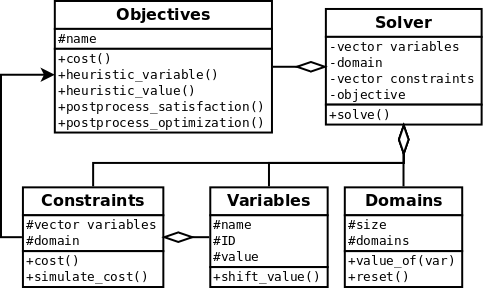
\includegraphics[width=\columnwidth]{figs/ghost.png}
  \caption{A simplified class diagram of \ghost}
  \label{fig:ghost}
\end{figure}
%--------------
\begin{figure}[th]
  \centering
  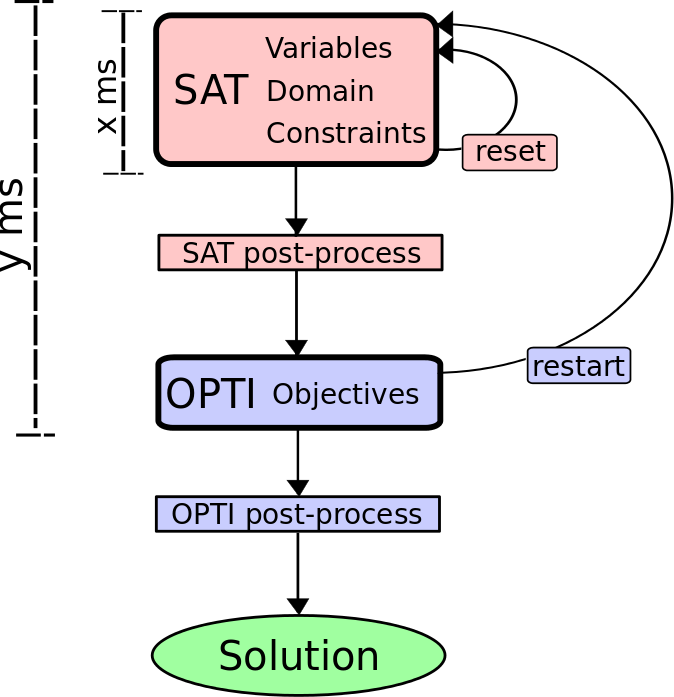
\includegraphics[width=\columnwidth]{figs/archi.png}
  \caption{\ghost architecture}
  \label{fig:archi}
\end{figure}
%--------------

There are only three parameters in  the solver: The two first ones are
temporal parameters. 


Even parameters Actually, experiments presented in the next sections shown
that no parameters  tuning is necessary to have  good performance: The
only  real parameter  of the  solver is  set to  a default  value that
leaded  to the  best results  in all  our experiments.  Of course,  it
remains possible to change this value by the developed user.


A developed user  has to build his own classes  upon theses first four
ones,  by inheriting  from  it. For  instance, to  create  a class  of
variables     representing     units,      this     is     done     by
\texttt{class~Unit~:~public~Variable}.   Classes  composed  for  other
classes, like \texttt{Domain} which need  to know on what variables it
will work with, must instantiate  the right templates. Thus, declaring
the   domain   for  the   target   selection   problem  is   done   by
\texttt{class~TargetDomain~:~public~Domain<Unit>}.

Concerning objective  functions, \ghost has been  designed to minimize
their  value.  If  a developer  user  needs to  maximize an  objective
function $f$,  this can be  simply adapted  to \ghost by  defining the
objective  function  $1/f$.   Our  solver is  designed  to  deal  with
mono-objective optimization problem only, thus, one can only choose at
most  one   objective  function  at   the  time  before   running  the
\texttt{solve}  function,  however  the   objective  function  can  be
dynamically changed between two calls of \texttt{solve}. The choice of
designing  a  mono-objective   solver  is  pragmatic:  Multi-objective
solvers are in  general significantly slower, since  dealing with more
complex problems.  Multi-objective solvers  are also more difficult to
implement, but one goal of \ghost is  to propose a solver both easy to
use and to extend by implementing  new problems, which are welcomed to
be integrated into \ghost to be available to anyone.

In the next three sections, we explain how we model a reactive control
problem, a  tactic problem  and a strategy  problem with  a respective
\csp/\cop, and  what results we  obtained by applying \ghost  on these
models.   We   would  like  to   stress  that  no   modifications,  no
optimizations of  the solver has  been done to manage  these different
problems:   The  core   of  the   solver,  \ie,   everything  in   the
\texttt{Solver} class, remains unchanged.   Even if post-processes are
defined  differently in  their respective  \texttt{Objective} classes,
the way they are included and called into the solver is rigorously the
same.

% \begin{figure*}
%   \begin{lstlisting}
% vector< Unit > variables = { ... }
% vector< UnitEnemy  > enemies  = {  ... }  //specific  to the target selection problem
% TargetSelectionDomain domain( variables.size(), &enemies );
% vector< shared_ptr<TargetSelectionConstraint> > vecConstraints
%       { make_shared<TargetSelectionConstraint>( &vec, &domain ) };
% shared_ptr<TargetSelectionObjective> objective =
%       make_shared<MaxDamage>();
% Solver<Unit, TargetSelectionDomain, TargetSelectionConstraint>
%       solver( &vec, &domain, vecConstraints, objective );
% solver.solve();
% \end{lstlisting}
%   \centering
%   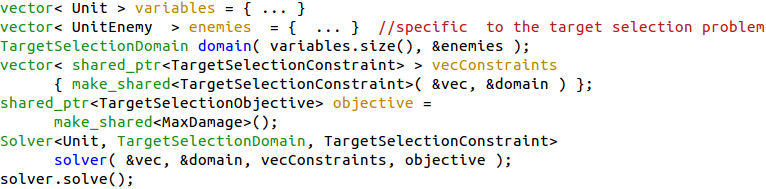
\includegraphics[width=\linewidth]{figs/solve.png}
%   \caption{Example  of  a  casual  use   of  \ghost,  for  the  target
%     selection problem}
%   \label{algo:casual}
% \end{figure*}

\section{Reactive control problem: The target selection}\label{sec:target}

Refer to Churchill  et al.~\cite{ChurchillSB12, ChurchillB12}, Uriarte
and Onta{\~n}{\'o}n~\cite{UriarteO12}

\subsection{Problem statement}

The  target   selection  problem  is  a   classical  reactive  control
problem. Its satisfaction  version is very easy, like it  is often the
case: It  consists of  assigning to  each unit of  a fighting  group a
reachable target, \ie, an enemy unit within our unit range.

In addition, one has also to take  into account a cooldown, that is to
say a fixed  number of StarCraft time $t$ within  a unit recharges and
has to  wait before shooting  again. This number  is the same  for all
units of  the same  type. We  can then  describe the  target selection
problem with the following \csp.

\modelcsp{the Target Selection problem}%
{A group of our units.}%
{A group of enemy units.}%
{Each living, ready-to-shoot  unit must aim a living  enemy within its
  range, if any.}

We have decided to model this  problem as a frame-by-frame problem: we
only consider the question ``what  enemy should I shoot this frame?'',
without  looking at  micro-management moves  like kiting,  \ie, moving
backward while recharging then attacking  forward when one is ready to
shoot.

Usually, RTS games  define specific characteristics to  each unit type
making the target selection more  subtle. Thus in StarCraft, each unit
type  has  a  size  (small,  medium   or  large)  and  a  damage  type
(concussive, normal  or explosive).  Table~\ref{tab:damage}  shows the
damage penalty  applied according the size  of the aimed unit  and the
damage type of  the shooter.  For instance, a normal  damage unit will
always  afflict  a  target  with  full  damage,  whatever  the  target
size. But a  concussive damage unit, like a Terran  Vulture, will only
make 5 damage points (without  counting upgrade neither armor) against
a large unit like a Terran Tank, instead of 20 damage points as usual.
%--------------
\begin{table}[!h]
  \caption{Damage efficiency matrix in StarCraft.}
  \label{tab:damage}
  \centering
  \begin{tabular}{|c|l|c|c|c|} 
    \cline{3-5}
    \multicolumn{2}{c|}{} & \multicolumn{3}{c|}{Damage type} \\ 
    \multicolumn{2}{c|}{} & \multicolumn{1}{c}{Concussive} & \multicolumn{1}{c}{Normal} & \multicolumn{1}{c|}{Explosive}\\
    \hline
    \multicolumn{1}{|c}{\multirow{3}{*}{\rotatebox[origin=c]{90}{size}}}& {\em Small} & 100\% & 100\% & 50\%\\
    \multicolumn{1}{|c}{} & {\em Medium} & 50\% & 100\% & 75\%\\
    \multicolumn{1}{|c}{} & {\em Large} & 25\% & 100\% & 100\%\\
    \hline
  \end{tabular}
\end{table}
%--------------
Moreover, some  units have a  splash attack, afflicting damage  to the
target's neighbors. In  StarCraft, two splash attack  types exist: the
linear splash, where the  unit can hit a line of  enemies, such as the
Zerg Lurker, and the radial splash  where an attack triggers a circled
wave shock hitting units around the target within one the three splash
radiuses. The  first radius  afflict 100\% of  damage, the  second one
50\% and the  last one 25\%.  Terran Firebat are  special cases mixing
both linear and radial splashes.

This,   combined  with   damage  efficiency,   leads  to   interesting
optimization  opportunities.   In  this  work,  we   investigated  two
different objective functions:
%--------------
\begin{itemize}
\item {\bf Max  damage}, where our group tries to  deal as much damage
  as possible within the current frame.
\item {\bf  Max kill},  where our  group tries to  kill as  much enemy
  units as possible within the current frame.
\end{itemize}
%--------------
Notice that these two objective are  more complex that looking for the
maximal damage  or maximal dead  enemies for each  unit independently:
Imagine a scenario where  we have two units U1 and  U2 and two enemies
E1 and E2,  such that U1 can afflict  10 damage points to E1  and 9 to
E2, U2 can afflict 8 damage points to  E1, but E2 is out of range, and
E1 has 5 hit points (HP) left.  The best global assignment is U1 to E2
and U2 to E1, even if U1 deals more damage to E1.

\subsection{\ghost results}

Figure~\ref{fig:target}   shows  the   mirror   setup   we  used   for
experiments. We chose  Terran units since many of  them are long-range
attack  units and  this make  things  more interesting  form a  target
selection point of  view. Also, we packed units close  each others, to
make significant the Terran Siege Tank's splash damage.
%--------------
\begin{figure}[!h]
  \centering
  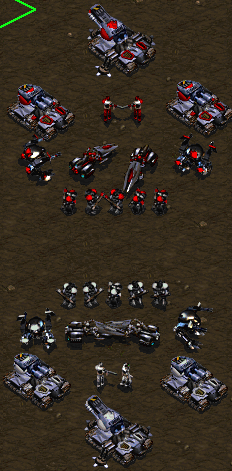
\includegraphics[width=0.7\columnwidth]{figs/target_setup.png}
  \caption{Mirror  Terran  unit  composition and  placement  used  for
    experiments. Line 1: 5 marines. Line  2: 2 Goliaths and 2 Vultures
    (in the middle). Line  3: 2 Siege Tanks in tank  mode and 2 Ghosts
    (in the middle). Line 4: 1  Siege Tank in siege mode, doing splash
    damage.}
  \label{fig:target}
\end{figure}
%--------------
Terran Firebat has not been taking into account in the small simulator
we wrote for testing \ghost on the target selection problem.  We first
planned    to    use   SparCraft~\cite{ChurchillB11,    ChurchillSB12,
  ChurchillB12}, but  we were lacking of  time to learn how  to use it
and combined  it with \ghost. It  was then faster to  develop an quick
ad-hoc simulator (about 200 lines of C++ code). 

The simulator is here to emulate a  combat of two unit groups and thus
need to trigger cooldowns, manage each unit HP, apply damages, compute
Euclidian  distances  between  units. Ranges,  damage  efficiency  and
splash damages  are directly  managed by \ghost.   It is  important to
stress that, in this simulator, enemy units are randomly shooting at a
reachable target.

What our simulator does not consider:
%--------------
\begin{itemize}
\item Healing, repair, HP or shield regeneration,
\item Terrain level (high/low ground),
\item Air shots (in StarCraft, there is always a small chance to miss
  the target),
\item Upgrades, Researches, Spells,
\item Friendly fire,
\item Firebats.
\end{itemize}
%--------------
\begin{table*}[ht]
  \caption{Average  results over  100 simulations  for both  objective
    functions, with the setup shown in Figure~\ref{fig:target}.}
  \label{tab:target}
  \centering
  \begin{tabular}{|l|c|c|c|c|c|c|} 
    \cline{4-7}
    \multicolumn{3}{c|}{} & \multicolumn{2}{c|}{\ghost victory} & \multicolumn{2}{c|}{Opponent victory}\\
    \hline
    {\em Objective} & Win \% & \# Draws & \# \ghost living units & \ghost HP &
    \# Opponent living units & Opponent HP\\
    \hline
    {\em Max Damage} & 92.0 & 2 & 3.6 & 191.7 & 1.0 & 46.5\\
    {\em Max Kill} & 79.0 & 4 & 3.6 & 203.0 & 1.1 & 83.6\\
    \hline
  \end{tabular}
\end{table*}
%--------------
We ran  100 simulations  for both objective  functions until  only one
group is completely  annihilated. Eventually, the two  groups can kill
one another, leading to a draw. We can then compute \ghost's win rate,
as well as the  average number of \ghost's living units  at the end of
the simulation and the average of remaining HP for \ghost living units
when \ghost wins, and the same averages when the opponent wins.

Table~\ref{tab:target}\footnote{All target experiment  results and the
  simulator            can            be           found            at
  \href{https://github.com/richoux/GHOST\_paper/tree/master/xp/target}{github.com/richoux/GHOST\_paper/tree/master/xp/target}}
shows that the Max Damage objective  wins 92\% of the time against the
mirror unit group shooting randomly. The Max Kill objective seems less
efficient with  a win rate of  79\%. One explanation is  that Max Kill
may not  be a heuristic  as good as Mas  Damage when enemy  units have
their full HP.  It would be  interesting to cross these two objectives
to see if it leads to better results.

For both objectives, we see that \ghost victories are undeniable, with
in average  3.6 remaining units  after the simulation,  whereas losses
are  tight,  with  just one  living  enemy  unit  at  the end  of  the
combat. The average of total remaining  HP is also clearly in favor of
\ghost.

\subsection{Future works}

To go further,  we could implement additional  objective functions for
the target selection  problem, like minimizing damage  waste, \ie, try
to be as close as 0 HP while killing an enemy unit instead of shooting
a 5-HP target with 20 damage points  for instance. Even if \ghost is a
mono-objective solver, we could craft new objectives by mixing already
encoded  ones,   by  simply  applying  a   priority  heuristics,  like
``maximize  killings  first,  and  consider  maximizing  damage  as  a
tiebreacker''.

Also, the  current implementation only  deal with Terran  ground units
for the target selection problem.  Extending it to all StarCraft units
would be easy.

Finally, improving the current simulator or using SparCraft would make
our  experiments sharper.   This could  even be  used in-game  to make
simulations through  Monte Carlo sampling,  and then help to  make the
decision about what unit to aim.

\section{Tactic problem: Wall-in}\label{sec:wall}
Refer to Certicky~\cite{Certicky13}, Richoux et al.~\cite{RichouxUO14}
\subsection{Problem statement}
\subsection{\ghost results}
%--------------
\begin{table*}[ht]
    \caption{Optimization   results   over  48   different   problems,
      extracted  form   7  different   maps  from  the   StarCraft  AI
      competition. Results are the average of 100 runs in each problem
      (total of 4800 runs per configuration).}
    \label{tab:wall}
    \centering
    \begin{tabular}{|l|c|c|c|}
      \cline{2-4}
      \multicolumn{1}{c|}{} & {\em Satisfaction run}& {\em Optimization run}& {\em Optimization run solved} \\
      \hline
      {\em Optimizing number of buildings (number of buildings)} 	& 4.05                  & 2.56                  & 98.04\% \\ 
      {\em Optimizing gaps (number of gaps)} 				& 1.32                  & 0.03                  & 97.50\%  \\ 
      {\em Optimizing tech-level (average tech level of buildings)} 	& 1.99                  & 1.35                 & 97.54\%  \\
      \hline
    \end{tabular}  
\end{table*}
%--------------
4800 runs, 4680 walls found, 4527 perfect walls (\ie, 96.73\% of walls
found)

Table~\ref{tab:wall}\footnote{All wall-in data  and experiment results
  can                   be                  found                   at
  \href{https://github.com/richoux/GHOST\_paper/tree/master/xp/wallin}{github.com/richoux/GHOST\_paper/tree/master/xp/wallin}}
shows

\subsection{Future works}


\section{Strategy problem: The build order}\label{sec:bo}

Refer   to   Churchill   and   Buro~\cite{ChurchillB11},   Kuchem   et
al.~\cite{KuchemPR13},  Weber   and  Mateas~\cite{WeberM09},   Cho  et
al.~\cite{ChoKC13}, Blackford~\cite{Blackford14}

\subsection{Problem statement}
A build  order planning is  a series  of actions following  a specific
timing, in order  to achieve a goal.  Such a goal is  a combination of
buildings,  units,  upgrades  and researches  produced.  Usually,  the
objective for a  player is to reach a fixed  goal the fastest possible
way. However, alternatives  can also be considered,  like reaching the
goal without sacrificing  the economy, or focussing first  on units in
order to have an army quickly available.

A  build order  planning can  be intuitively  modeled by  a \csp  as a
permutation problem,  where a bijection  maps the set of  variables to
the  domain. Changing  the  value  of one  variable  is then  actually
swapping its value with another variable.

All  actions have  a (potentially  empty) dependencies  list, \ie,  an
action  $\alpha$  has a  list  of  actions  that are  required  before
starting  $\alpha$.  For  instance, to  start the  \textit{Air Weapons
  Upgrade level  2}, it is  required to have finished  the \textit{Air
  Weapons Upgrade level  1}. Notice that we can  dive recursively into
these  dependencies  list. Thus  if  someone  aims to  do  \textit{Air
  Weapons  Upgrade  level  2}  for Protoss,  it  required  \textit{Air
  Weapons    Upgrade   level    1},    which    requires   itself    a
\textit{Cybernetics Core}, which requires a \textit{Gateway}.

The \csp model we propose for  the build order planning problem is the
following one:

\modelcsp{the Build Order Planning problem}%
{All actions we need to reach our goal.}%
{Order of actions.}%
{Each dependency of an action $\alpha$ must occurs before $\alpha$.}

\subsection{\ghost results}
%--------------
\begin{table*}[ht]
  \caption{Average  makespan  of Humans  and  \ghost  build orders  in
    StarCraft time over 3647 games.}
  \label{tab:bo}
  \centering
  \begin{tabular}{|l|c|c|c|c|} 
    \hline
    \multicolumn{5}{|c|}{Games till 10.000 frames} \\ 
    \hline
    {\em Match-up} & Humans & \ghost & \% solved &
    Gain \\ 
    \hline
    {\em All} & 656.02 & 619.62 & 94.4 & 36.40\\
    {\em PvP} & 651.51 & 608.06 & 95.0 & 43.45\\
    {\em PvT} & 660.50 & 628.17 & 93.9 & 32.33\\
    {\em PvZ} & 649.20 & 609.34 & 95.0 & 39.86\\
    \hline
  \end{tabular}
  %\hfill  
  \begin{tabular}{|l|c|c|c|c|} 
    \hline
    \multicolumn{5}{|c|}{Games till 7.800 frames} \\ 
    \hline
    {\em Match-up} & Humans & \ghost & \% solved &
    Gain \\ 
    \hline
    {\em All} & 522.50 & 491.11 & 98.8 & 31.39\\
    {\em PvP} & 516.08 & 485.56 & 99.3 & 30.52\\
    {\em PvT} & 527.66 & 506.65 & 98.3 & 21.01\\
    {\em PvZ} & 515.81 & 458.23 & 99.7 & 57.58\\ 
    \hline
  \end{tabular}  
\end{table*}
%--------------
For  Table~\ref{tab:bo}\footnote{All  build   order  data,  experiment
  results     and     the     simulator    can     be     found     at
  \href{https://github.com/richoux/GHOST\_paper/tree/master/xp/build\_order}{github.com/richoux/GHOST\_paper/tree/master/xp/build\_order}},
\ghost has been run 10 times on each game. We also analyzed replays of
games played by top Korean pro-gamers,  \ie, Kim "Bisu" Taek Yong, Doh
"BeSt" Jae  Wook, Woo  "Violet" Jung  Ho, Yang  "Cure" Jung  Hyun, all
Protoss players, against Lee "Flash"  Young Ho (Terran), Lee "Jaedong"
Jae Dong  (Zerg), Ma "sAviOr"  Jae Yoon  (Zerg) and match  their build
orders with \ghost \todonote{[Flo] no data here, but I can put them}.

Computation time is  only 20ms for satisfaction runs and  30ms for the
(global) optimization run. This means that \ghost can compute a highly
optimized build order within one StarCraft frame only.

Why planing a build  order is easier than wall-in? A  huge part of the
answer is  that planing  a build  order can  be modeled  in \csp  by a
permutation  problem,  which  drastically decrease  the  combinatorial
complexity of the problem.

Set up: Churchill and  Buro~\cite{ChurchillB11} gives too advantageous
set up.  Based on the analysis  of games from Korean pro-gamers listed
above, we parameterized our simulator as follow (in StarCraft time t):
%--------------
\begin{itemize}
\item Time to go build something: 5t (4t in \cite{ChurchillB11})
\item Time to go back  gathering minerals after building something: 4t
  (0 in \cite{ChurchillB11})
\item Time to go from the base  to mineral patches to start mining: 5t
  (0 in \cite{ChurchillB11})
\item  Time for  a probe  to  switch from  mineral  to gas:  5t (0  in
  \cite{ChurchillB11})
\item Mineral gathering  rate: 0.68 mineral per worker per  t (1.07 in
  \cite{ChurchillB11})
\item  Gas  gathering  rate:  1.15  gas per  worker  per  t  (1.66  in
  \cite{ChurchillB11})
\end{itemize}  
%--------------

\subsection{Future works}


\section{Conclusion}\label{sec:conclusion}





%\section*{Acknowledgments} {\color{blue} This research is partially funded by projects ... and ... . }



% Can use something like this to put references on a page
% by themselves when using endfloat and the captionsoff option.
\ifCLASSOPTIONcaptionsoff
  \newpage
\fi

%\begin{thebibliography}{1}
%\end{thebibliography}
\bibliographystyle{IEEEtran}                                                    
\bibliography{ghost}

%\begin{IEEEbiographynophoto}{FirstName LastName}
%Biography text here.
%\end{IEEEbiographynophoto}

%\begin{IEEEbiography}[{\includegraphics[width=2cm, keepaspectratio]{jim.jpg}}]{Jim Raynor}
%Jim Raynor was a Confederate marshal on Mar Sara at the time of the first zerg incursions on that world. He is now with Raynor's Raiders Inc.
%\end{IEEEbiography}


%\begin{IEEEbiography}[{\includegraphics[width=2cm, keepaspectratio]{figures/santi.jpg}}]{Santiago Onta\~{n}\'{o}n}

% \begin{IEEEbiographynophoto}{Florian Richoux}
%   is an associate  professor at the Laboratory of  Computer Science of
%   the University of Nantes,  France.  His main research field concerns
%   parallel  algorithms for solving  constraint-based problems  and has
%   strong  interests   in  AI,  in  particular  game   AI  and  machine
%   learning. He  obtained his Ph.D. in Theoretical  Computer Science at
%   the {\'E}cole Polytechnique  in 2009 and has been  for three years a
%   CNRS   research  fellow  at   the  Japanese-French   Laboratory  for
%   Informatics of the University of Tokyo, Japan.
% \end{IEEEbiographynophoto}


% \begin{IEEEbiographynophoto}{Alberto Uriarte}
% received the B.S. degree in Computer Science from Autonomous University of Barcelona (UAB), Spain, in 2006 and the M.S. degree in Computer Vision and Artificial Intelligence from Autonomous University of Barcelona (UAB), Spain, in 2011. He is currently pursuing the Ph.D. degree in computer science at Drexel University. His research interest includes game AI, RTS games, multiagents systems, procedural content generation, computational geometry, machine learning and drama management.  
% \end{IEEEbiographynophoto}

\end{document}


In his AIIDE 2010 keynote, Chris Jurnet described the technique XXX, implemented by [COMPANY] in the game YYY \cite{gameurl}
